\let\negmpace\undefined
\let\negthickspace\undefined
\documentclass[journal]{IEEEtran}
\usepackage[a5paper, margin=10mm, onecolumn]{geometry}
%\usepackage{lmodern} % Ensure lmodern is loaded for pdflatex
\setlength{\headheight}{1cm} % Set the height of the header box
\setlength{\headsep}{0mm}     % Set the distance between the header box and the top of the text
\usepackage{xparse}
\usepackage{gvv-book}
\usepackage{gvv}
\usepackage{cite}
\usepackage{amsmath,amssymb,amsfonts,amsthm}
\usepackage{algorithmic}
\usepackage{graphicx}
\usepackage{textcomp}
\usepackage{xcolor}
\usepackage{txfonts}
\usepackage{listings}
\usepackage{enumitem}
\usepackage{mathtools}
\usepackage{gensymb}
\usepackage{comment}
\usepackage[breaklinks=true]{hyperref}
\usepackage{tkz-euclide} 
\usepackage{listings}
% \usepackage{gvv}                                        
\def\inputGnumericTable{}                                 
\usepackage[latin1]{inputenc}                                
\usepackage{color}                                            
\usepackage{array}                                            
\usepackage{longtable}                                       
\usepackage{calc}                                             
\usepackage{multirow}                                         
\usepackage{hhline}                                           
\usepackage{ifthen}                                           
\usepackage{lscape}
\renewcommand{\thefigure}{\theenumi}
\renewcommand{\thetable}{\theenumi}
\setlength{\intextsep}{10pt} % Space between text and floats
\numberwithin{equation}{enumi}
\numberwithin{figure}{enumi}
\renewcommand{\thetable}{\theenumi}
\begin{document}
\bibliographystyle{IEEEtran}
\title{Question-7-7.2-8}
\author{EE24BTECH11033 - KOLLURU SURAJ}
% \maketitle
% \newpage
% \bigskip
{\let\newpage\relax\maketitle}
\textbf{Question}:\\
The centre of circle is $\myvec{2a\\a-7}$. Find the values of $a$ if the circle passes through the point $\vec{A}\myvec{11\\-9}$and has diameter $10\sqrt{2}$ units 
\\
\solution \\
\begin{table}[!ht]
  \centering
  \begin{tabular}{ |c| c|}
    \hline
    \textbf{point}  &  \textbf{Coordinates}\\
    \hline
    $\vec{A}$ & $\brak{-4,6}$ \\
    \hline
    $\vec{B}$ & $\brak{-4,-6}$\\
    \hline
    $\vec{C}$ & $\brak{-4,2}$\\
    \hline
\end{tabular}    


  \caption{variables used}
\end{table}\\
The radius of circle is $\frac{diameter}{2}$
\begin{align}
    \implies radius=5\sqrt{2}
    \end{align}
     The equation of a circle is given by 
	
\begin{align}
	\norm{\vec{x}}^2 + 2 \vec{u}^{\top}\vec{x} + f = 0
\end{align}
for
		\begin{align}
	 \vec{u}=-\vec{c}, f = \norm{\vec{c}}^2-r^2
		\end{align}
  Now,
  \begin{align}
      \vec{u}=-\myvec{2a\\a-7},f=5a^2-14a-1
  \end{align}
  On substituting $x$=$\myvec{11\\-9}$
  \begin{align}
  202-26a-126+5a^2-14a-1=0\\
  5a^2-40a+75=0\\
  a^2-8a+15=0\\
  a=3,a=5
  \end{align}
  \begin{figure}[h!]
   \centering
   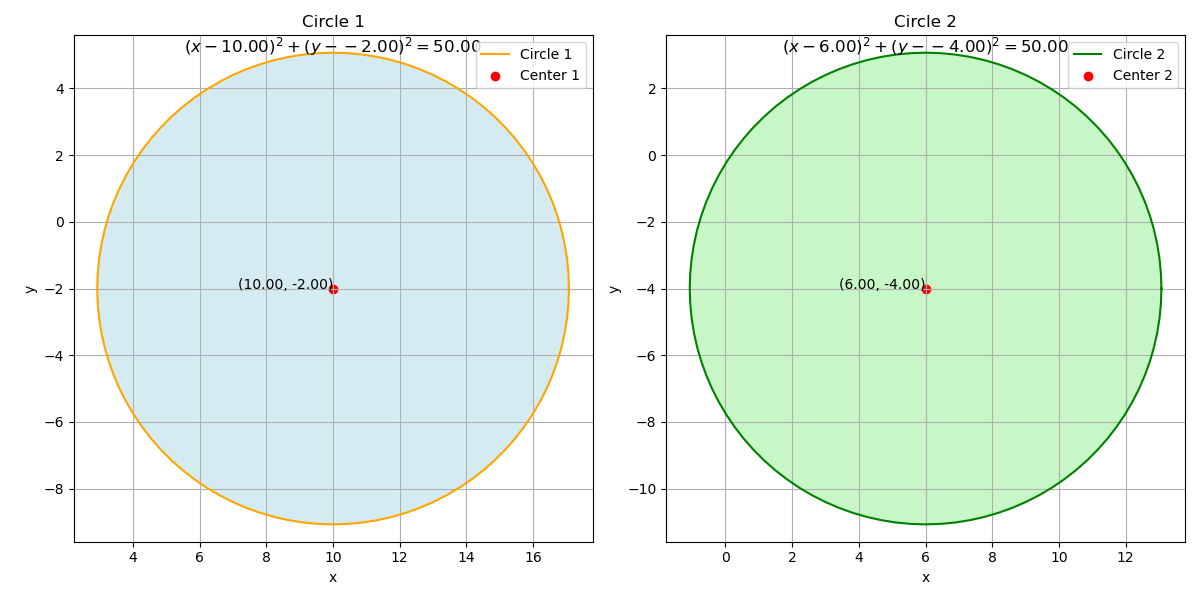
\includegraphics[width=0.7\linewidth]{figs/Figure_1.png}
   
   \label{stemplot}
\end{figure}

\end{document}
